\documentclass{llncs}
\usepackage{times}
\usepackage[T1]{fontenc}

% Comentar para not MAC Users
%\usepackage[applemac]{inputenc}

\usepackage{a4}
%\usepackage[margin=3cm,nohead]{geometry}
\usepackage{epstopdf}
\usepackage{indentfirst}
\usepackage{graphicx}
\usepackage{float}
\usepackage{fancyvrb}
\usepackage{amsmath}
%\renewcommand{\baselinestretch}{1.5}

\begin{document}
\mainmatter
\title{TP2: Protocolo IPv4}

\titlerunning{TP2: Protocolo IPv4}

\author{Diogo Braga \and João Silva \and Ricardo Caçador}

\authorrunning{Diogo Braga \and João Silva \and Ricardo Caçador}

\institute{
University of Minho, Department of  Informatics, 4710-057 Braga, Portugal\\
e-mail: \{a82547,a82005,a81064\}@alunos.uminho.pt\\
PL4, Grupo 7
}

\date{}
\bibliographystyle{splncs}

\maketitle

\section{Captura de tráfego IP}

\subsection{Exercício 1}
\emph{Prepare uma 
topologia CORE
para  verificar o comportamento  do traceroute. Ligue um host (pc) h1 a um
router r2; o router r2 a um router r3, que por sua vez, se liga a um host  (servidor) s4. (Note  que  pode  não existir conectividade  IP imediata entre h1 e s4 até que o routing estabilize).
Ajuste  o  nome  dos 
equipamentos atribuídos por defeito para a topologia do enunciado.}

\begin{figure}
\begin{center}
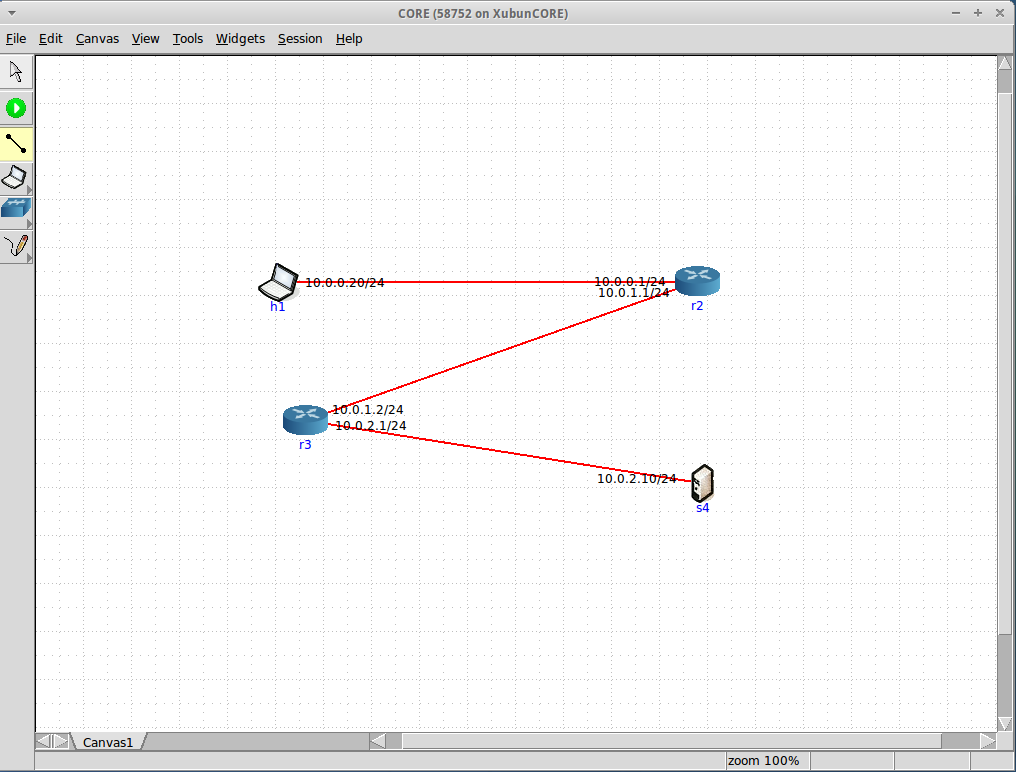
\includegraphics[scale=0.30]{intro.png} 
\end{center}
\caption{\label{fig:intro}Rede do exercício 1 do enunciado.}
\end{figure} 

\subsubsection{a.}
\emph{Active o wireshark ou o tcpdump no pc h1. Numa shell de h1, execute o comando traceroute-I para o endereço IP do host s4. }

\begin{figure}[H]
\begin{center}
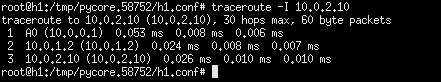
\includegraphics[scale=0.54]{traceroute_a.png} 
\end{center}
\caption{\label{fig:shellh1}Shell de h1 com comando traceroute.}
\end{figure} 
\par
\textbf{R:} Como se pode observar na figura \ref{fig:shellh1}, os pacotes passam por 2 routers, cujos IPs das interfaces ativas de cada um são, respetivamente, 10.0.0.1 e 10.0.1.2, até chegarem ao destino cujo IP da sua interface ativa é 10.0.2.10.

\subsubsection{b.}
\emph{Registe  e  a
nalise  o  tráfego
ICMP 
enviado
por  h
1
e 
o  tráfego  ICMP 
recebido
como
resposta. C
omente
os resultados
face 
ao comportamento 
esperado.}

\begin{figure}[H]
\begin{center}
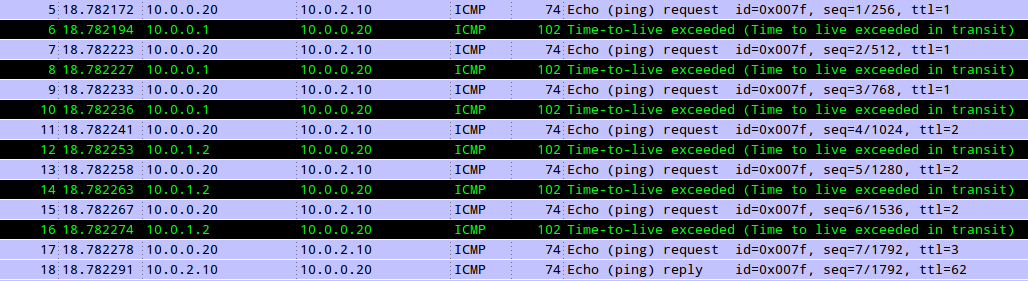
\includegraphics[scale=0.40]{trafego_b.png} 
\end{center}
\caption{\label{fig:trafego_b}Tráfego capturado pelo Wireshark.}
\end{figure} 
\textbf{R:} Como predefinição o traceroute envia 3 datagramas com o mesmo TTL pelo que capturamos 3 vezes mais mensagens ICMP. 
De modo a simplificar utilizamos o comando \emph{"traceroute -I 10.0.2.10 -q 1"} que apenas envia um datagrama, facilitando a análise do tráfego.
\begin{figure}[H]
\begin{center}
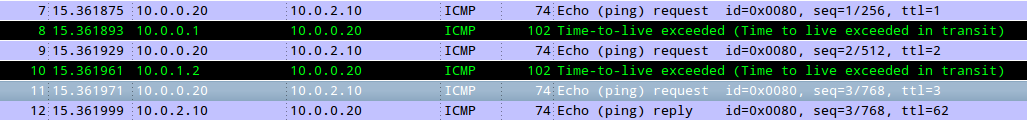
\includegraphics[scale=0.40]{trafego_b2.png} 
\end{center}
\caption{\label{fig:trafego_b2}Tráfego capturado pelo Wireshark.}
\end{figure}

Analisando o tráfego percebe-se que são enviadas duas mensagens do tipo \emph{Time-to-live exceeded} de cada um dos routers para h1. Já se esperava este resultado uma vez que o traceroute é um processo iterativo que permite descobrir a rota até ao destino "salto-a-salto".
As mensagens ICMP são enviadas para h1 quando o TTL é 1 e 2, respetivamente, pelo primeiro router (10.0.0.1) e pelo segundo router (10.0.1.2).Neste caso o TTL é excedido.
Como esperado quando o TTL é 3, o datagrama já chega ao destino e o destino responde como se pode verificar na última linha da figura \ref{fig:trafego_b2}.


\subsubsection{c.}
\emph{Qual  deve  ser  o  valor 
inicial 
mínimo
do  campo  TTL  para  alcançar  o 
destino 
s
4
? 
Verifique na prática que a sua resposta está correta.}

\textbf{R:} O valor mínimo do campo TTL para alcançar o destino s4 deve ser 3, uma vez que o TTL é decrementado aquando da passagem em cada router. Para verificar este valor utilizamos o comando  \emph{"traceroute -I 10.0.2.10 -f 3"} que define o valor do primeiro TTL a ser usado como 3. Pela análise de tráfego da figura \ref{fig:shell_c} percebe-se que o datagrama atinge o destino logo na primeira tentativa.
\begin{figure}
\begin{center}
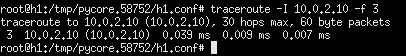
\includegraphics[scale=0.54]{shell_c.png} 
\end{center}
\caption{\label{fig:shell_c}Shell de h1 com comando traceroute.}
\end{figure}

\subsubsection{d.}
\emph{Qual o 
valor
médio 
do tempo de ida
-
e
-
volta (Round
-
Trip T
ime)
obtido
? }

\begin{figure}[H]
\begin{center}
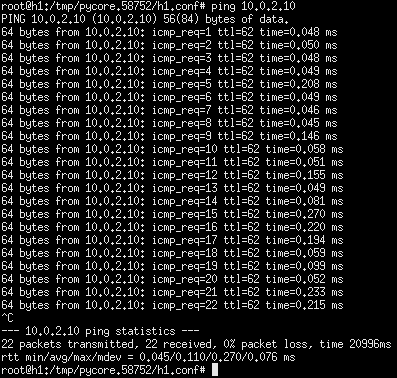
\includegraphics[scale=0.54]{shell_d.png} 
\end{center}
\caption{\label{fig:shell_d}Shell de h1 com comando ping.}
\end{figure}

\textbf{R:} Como se pode verificar pela figura \ref{fig:shell_d}, na penúltima linha estão os valores do Round-Trip Time (rtt), e o valor correspondente ao valor médio é o avg (\emph{average}), que é \textbf{0.110 milisegundos}.

\subsection{Exercício 2}
\emph{Procedimento a seguir: Usando o wireshark capture o tráfego gerado pelo traceroute para os seguintes tamanhos de pacote: (i) sem especificar, i.e., usando o tamanho por defeito; e (ii) 35XX bytes, em que XX é o seu número de grupo. Utilize como máquina destino o host marco.uminho.pt. Pare a captura. Com base no tráfego capturado, identifique os pedidos ICMP Echo  Request e o conjunto de mensagens devolvidas em resposta a esses pedidos. Selecione a primeira mensagem ICMP capturada (referente a (i) tamanho por defeito) e centre a análise no nível protocolar IP (expanda o tab correspondente na janela de detalhe do wireshark). Através da análise do cabeçalho IP diga: }

\begin{figure}[H]
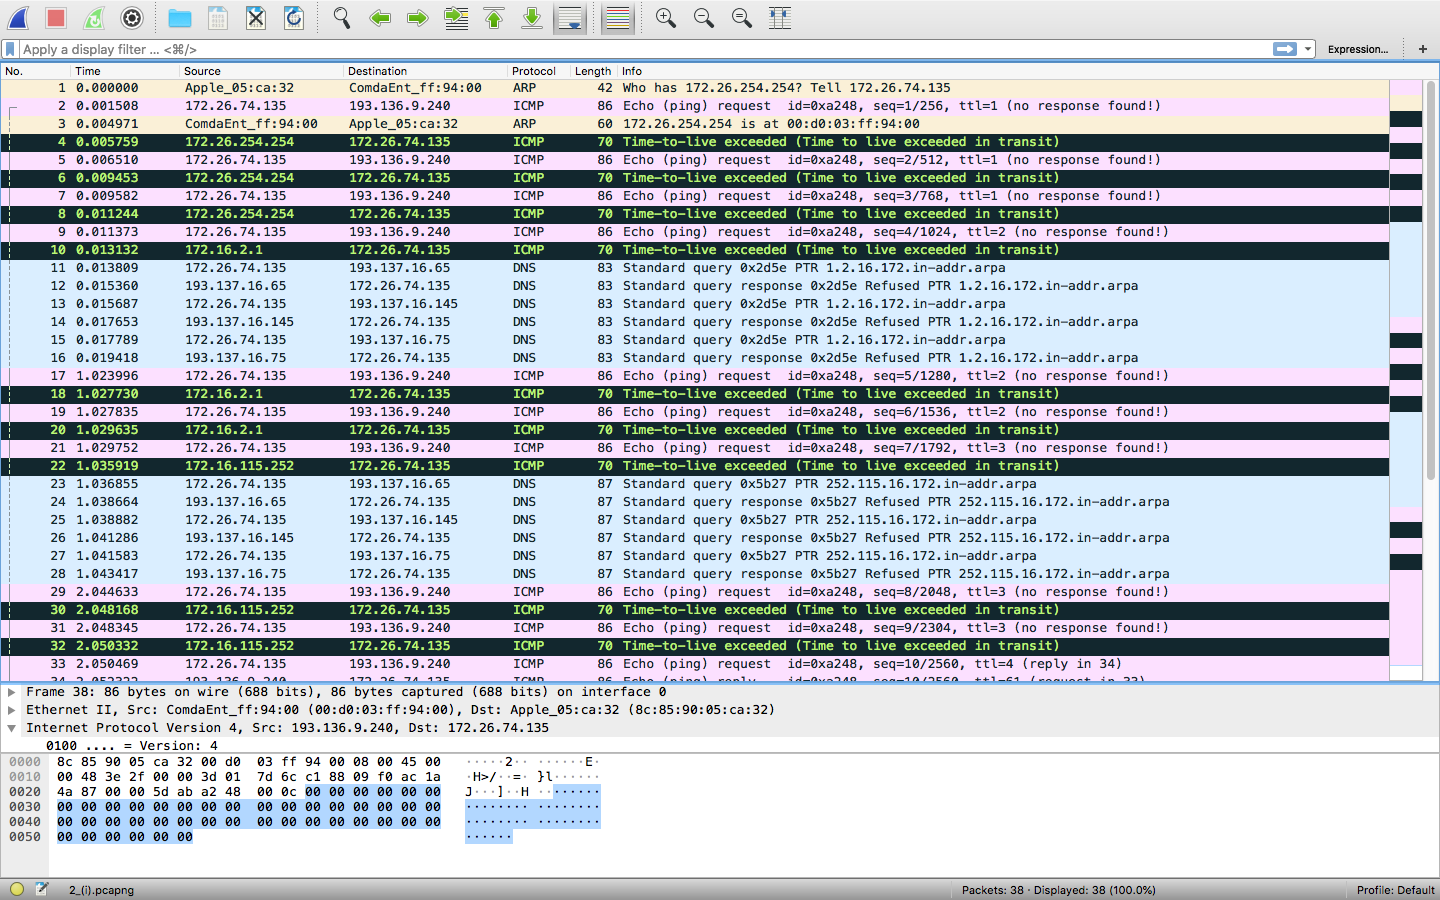
\includegraphics[scale=0.30]{2.png} 
\caption{\label{fig:2}Visão geral do tráfego gerado pelo traceroute usando o tamanho por defeito.}
\end{figure}

\subsubsection{a.}
\emph{Qual é o endereço IP da interface ativa
do 
seu computador?}

\begin{figure}
\begin{center}
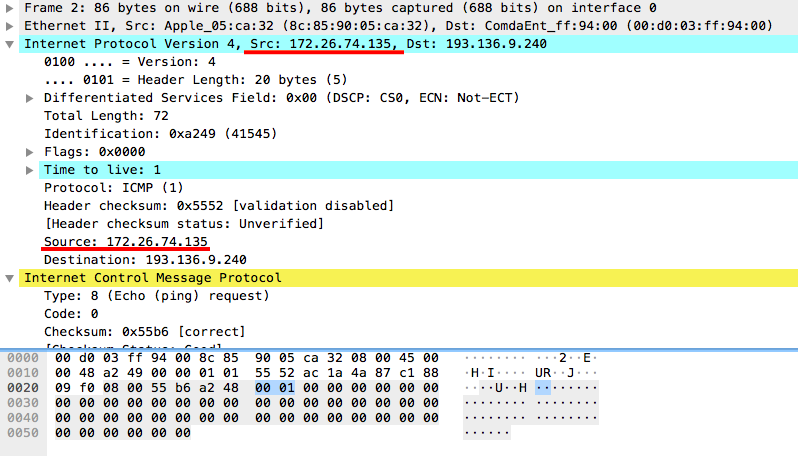
\includegraphics[scale=0.45]{2_a.png} 
\end{center}
\caption{\label{fig:2_a}Endereço IP da interface ativa do computador, sublinhado a vermelho.}
\end{figure}

\textbf{R:} Selecionando a primeira mensagem ICMP capturada, é atingida a janela presente na figura \ref{fig:2_a}. Nesta janela é possível observar a secção do IPv4 com o endereço IP da interface ativa do nosso computador, \textbf{172.26.74.135}. 

Concluimos que é este o endereço pois na secção do ICMP é possível visualizar que esta mensagem possui tipo 8. O tipo 8 descreve a mensagem de \textbf{echo request}. Este género de mensagem é um utilitário que usa o protocolo ICMP para testar a conectividade entre equipamentos. Consiste no envio de pacotes para o equipamento de destino e na captura das respostas. Se o equipamento de destino estiver ativo, uma "resposta" será devolvida ao computador solicitante. Por isso, concluimos que o nosso computador é o Source desta mensagem.

\subsubsection{b.}
\emph{Qual é o valor do 
campo 
protocolo
? O
que identifica
?}

\textbf{R:} Como se pode observar na figura \ref{fig:2_b}, o valor do campo protocolo é \textbf{ICMP (1)}. Este campo identifica o protocolo usado para a transmissão do datagrama. Neste caso, o ICMP (Internet Control Message Protocol) é usado para testar a conectividade entre a origem e o destino.

\begin{figure}[H]
\begin{center}
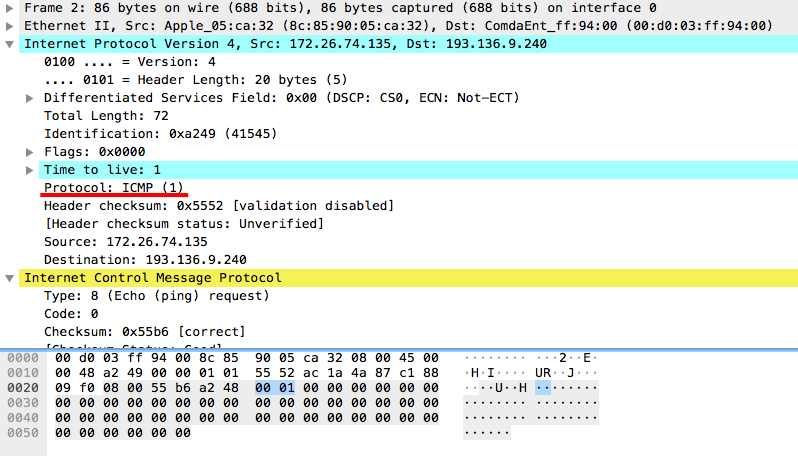
\includegraphics[scale=0.45]{2_b.png} 
\end{center}
\caption{\label{fig:2_b}Valor do campo protocolo, sublinhado a vermelho.}
\end{figure}

\subsubsection{c.}
\emph{Quantos bytes
tem o cabeçalho IP
(v4)
? Quantos 
bytes
tem o
campo de 
dados
(payload) 
do datagrama? 
Como 
se 
calcula
o tamanho do 
payload
?}

\textbf{R:} Os bytes do cabeçalho IP(v4) podem ser visualizados na figura \ref{fig:2_c} sublinhado a vermelho, neste caso \textbf{20 bytes}. O payload é parte principal dos dados transmitidos, da qual se excluem as informações utilizadas para, por exemplo, realizar a entrega, como cabeçalhos. Os bytes do payload são calculados subtraindo o número de bytes totais do datagrama (na figura \ref{fig:2_c} sublinhado a laranja) pelo número de bytes do cabeçalho antes mencionado. Portanto, o número de bytes do payload são (72 - 20 =) \textbf{52 bytes}.

\begin{figure}[H]
\begin{center}
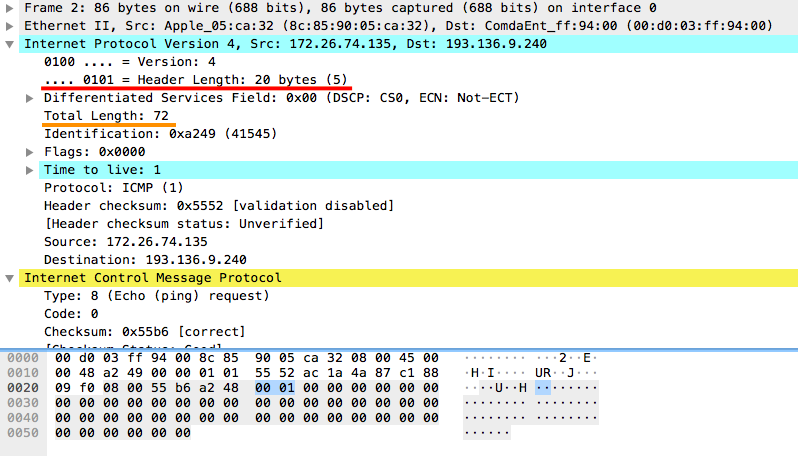
\includegraphics[scale=0.45]{2_c.png} 
\end{center}
\caption{\label{fig:2_c}Bytes do cabeçalho IP(v4) sublinhado a vermelho; Bytes totais do datagrama sublinhado a laranja.}
\end{figure}

\subsubsection{d.}
\emph{O
datagrama
IP
foi 
fragmentado
?
Justifique.}

\begin{figure}[H]
\begin{center}
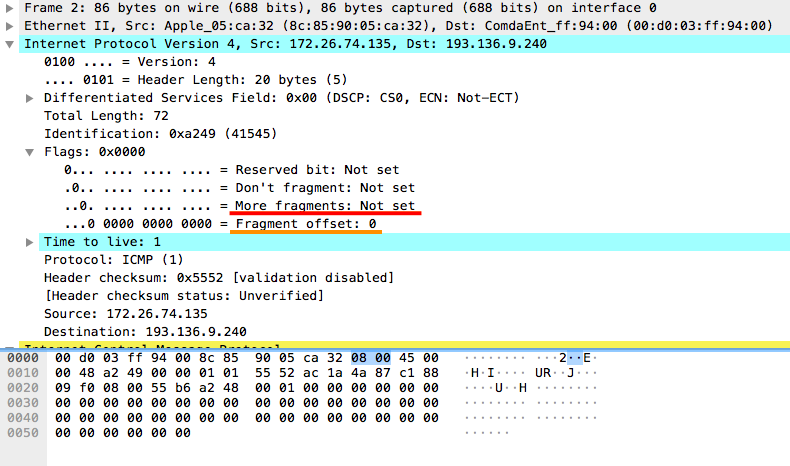
\includegraphics[scale=0.45]{2_d.png} 
\end{center}
\caption{\label{fig:2_d}Parâmetro de fragmentação sublinhado a vermelho; Offset do fragmento sublinhado a laranja.}
\end{figure}
\textbf{R:} Como se pode observar na figura \ref{fig:2}, não se verificam ações de fragmentação do datagrama. Caso existisse fragmentação seria possível de visualizar em ações consecutivas com datagramas fragmentados. Este facto pode ser confirmado mais especificamente na figura \ref{fig:2_d}, pois verifica-se que o parâmetro \textbf{More fragments} sublinhado a vermelho não está estabelecido (Not set). Visto não existir fragmentação, também o parâmetro offset do fragmento está a 0.

\subsubsection{e.}
\emph{Ordene os pacotes capturados de acordo com o endereço IP fonte (
e.g.,
selecionando 
o  cabeçalho  da  coluna 
Source
),  e 
analise  a  sequência  de 
tráfego ICMP
gerado a partir
do endereço 
IP 
atri
buí
do à
interface da 
sua 
máquina
.
Para  a
sequência
de  mensagens 
ICMP 
enviadas  pelo  seu 
computador, indique que campos do cabeçalho IP variam de pacote para 
pacote.}

\begin{figure}[H]
\begin{center}
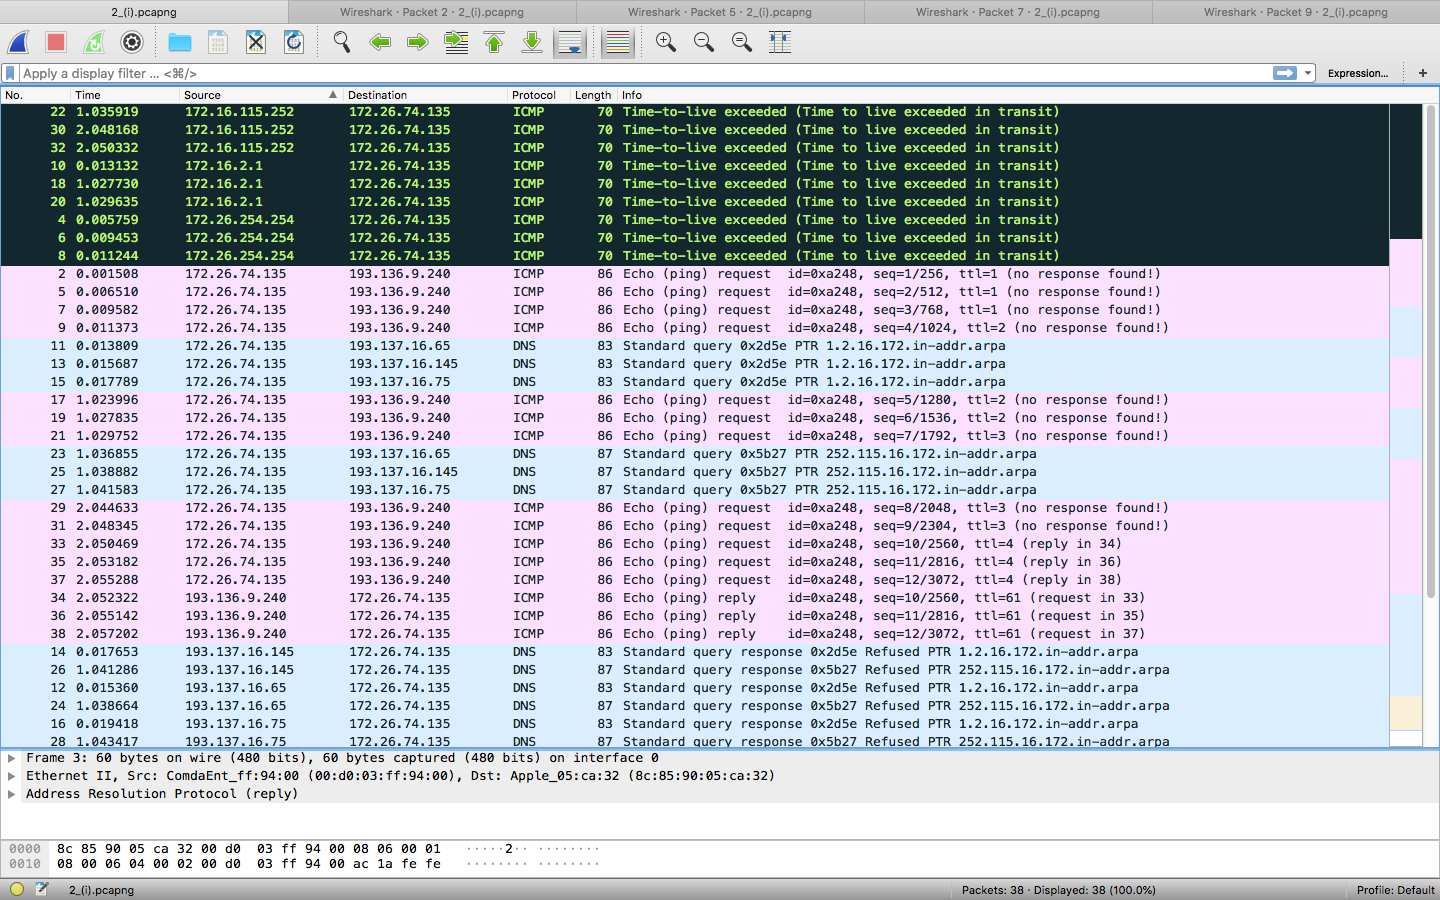
\includegraphics[scale=0.30]{2_e.png} 
\end{center}
\caption{\label{fig:2_e}Visão geral do tráfego gerado pelo traceroute ordenado de acordo com o endereço IP fonte.}
\end{figure}

\begin{figure}[H]
\begin{center}
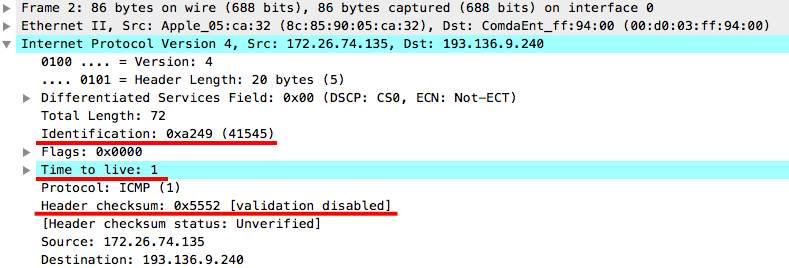
\includegraphics[scale=0.45]{2_e_1.png} 
\end{center}
\caption{\label{fig:2_e_1}Frame 2.}
\end{figure}

\begin{figure}[H]
\begin{center}
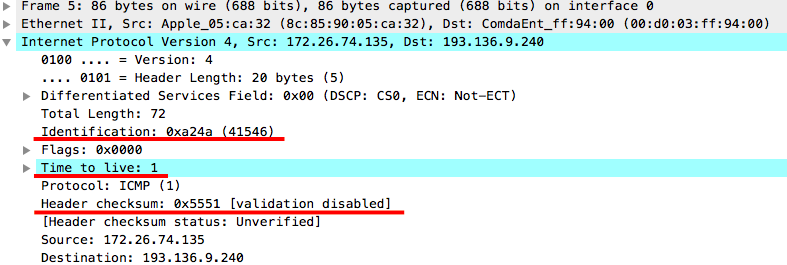
\includegraphics[scale=0.45]{2_e_2.png} 
\end{center}
\caption{\label{fig:2_e_2}Frame 5.}
\end{figure}

\begin{figure}[H]
\begin{center}
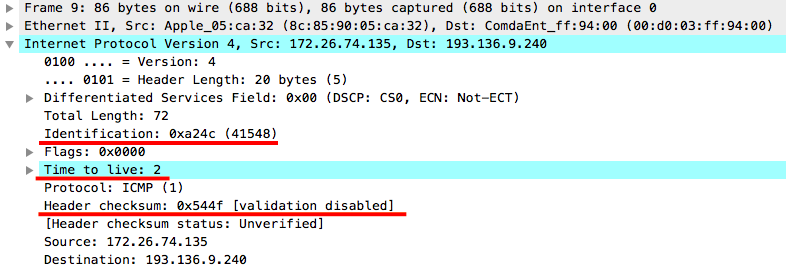
\includegraphics[scale=0.45]{2_e_3.png} 
\end{center}
\caption{\label{fig:2_e_3}Frame 9.}
\end{figure}

\textbf{R:} Tendo em vista os sublinhados das figuras \ref{fig:2_e_1}, \ref{fig:2_e_2} e \ref{fig:2_e_3}, é possível concluir que os campos do cabeçalho IP que variam de pacote para pacote são o campo \textbf{Identification}, o campo \textbf{Header Checksum} e o campo \textbf{Time to live} na secção do IP.

\subsubsection{f.}
\emph{Observa  algum 
padrão  nos  valores  do  campo  de  Identificação  do 
datagrama IP
e TTL
?}

O campo de identificação do datagrama IP aumenta uma unidade por cada datagrama enviado pelo nosso computador. Relativamente ao campo TTL, como usamos o comando traceroute padrão, ele envia 3 datagramas com o mesmo TTL pelo que o TTL aumenta uma unidade em cada 3 datagramas enviados pelo nosso computador. Por exemplo, tendo em conta os frames 2,5,7 e 9, é possível verificar nas imagens \ref{fig:2_e_1}, \ref{fig:2_e_2} e \ref{fig:2_e_3}, que o 2 e 5 têm o mesmo TTL, já o 9 tem um TTL maior uma unidade.

\subsubsection{g.}
\emph{Ordene o tráfego
capturado
por endereço 
destino
e
encontre a série de 
respostas  ICMP  TTL
exceeded
enviadas  ao  seu  computador
.  Qual  é  o 
valor  do  campo
TTL?
Esse
valor
permanece
cons
tante
para
todas  as 
mensagens  de  resposta
ICMP  TTL
exceeded
enviados  ao  seu 
host
? 
Porquê
?}

\begin{figure}[H]
\begin{center}
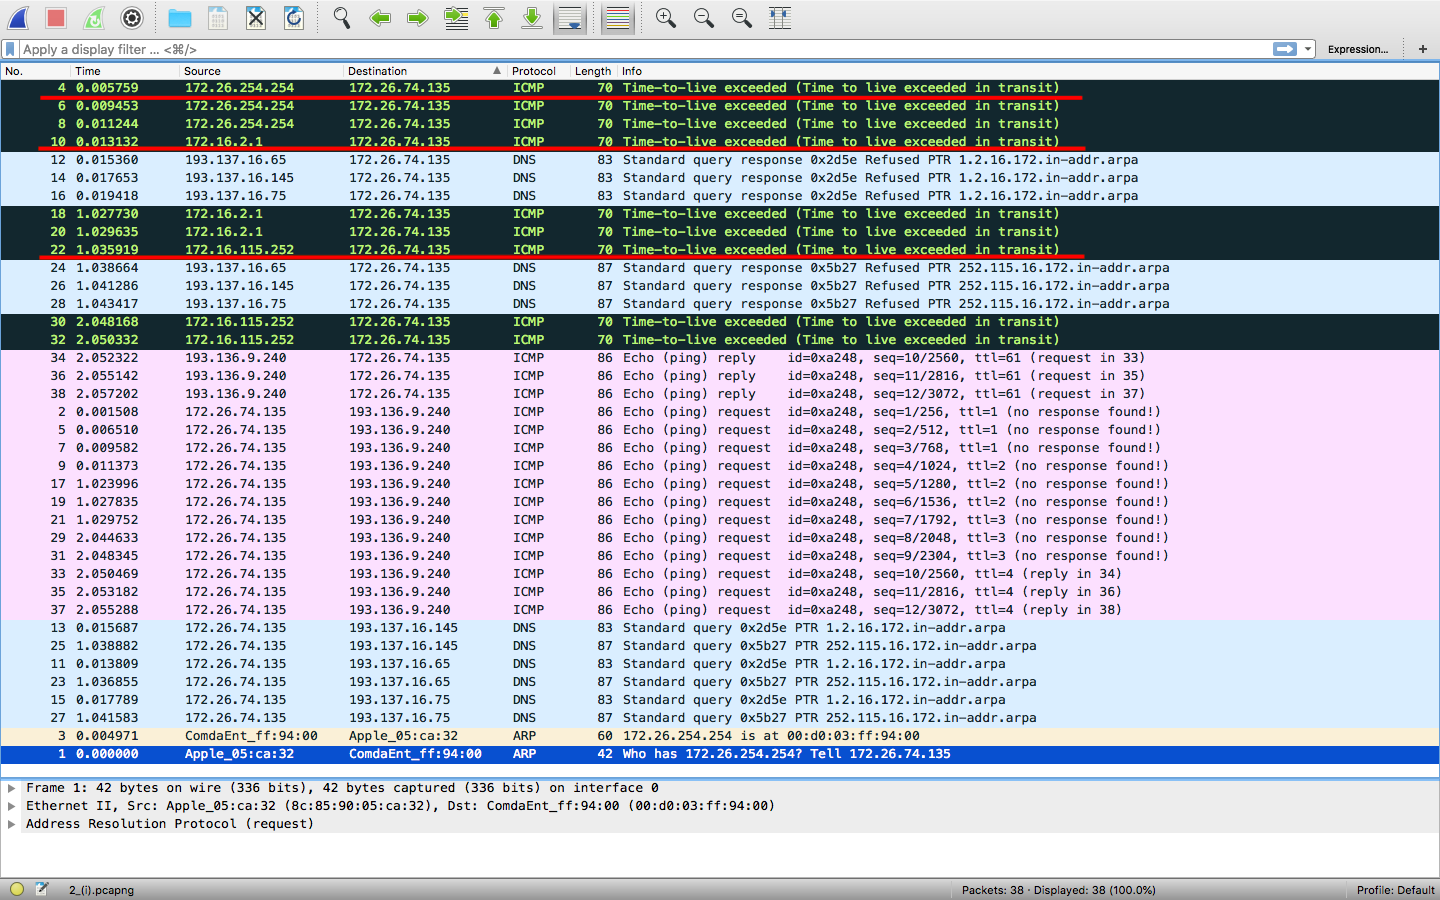
\includegraphics[scale=0.30]{2_g.png} 
\end{center}
\caption{\label{fig:2_e}Visão geral do tráfego gerado pelo traceroute ordenado por endereço destino.}
\end{figure}

\begin{figure}[H]
\begin{center}
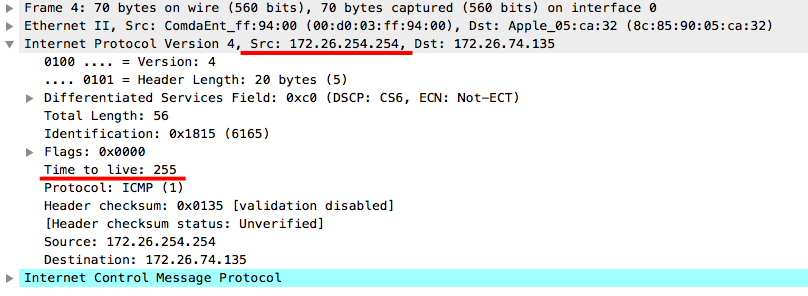
\includegraphics[scale=0.45]{2_g_1.png} 
\end{center}
\caption{\label{fig:2_g_1}Frame 4.}
\end{figure}

\begin{figure}[H]
\begin{center}
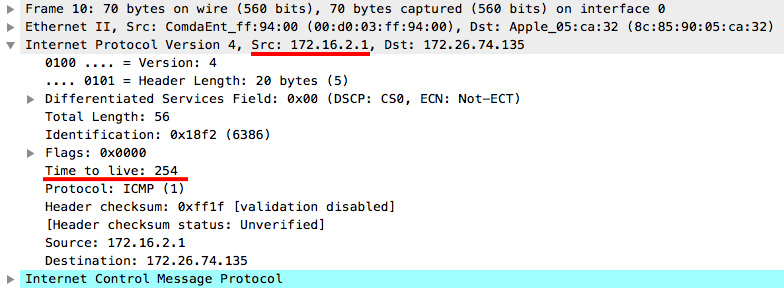
\includegraphics[scale=0.45]{2_g_2.png} 
\end{center}
\caption{\label{fig:2_g_2}Frame 10.}
\end{figure}

\begin{figure}[H]
\begin{center}
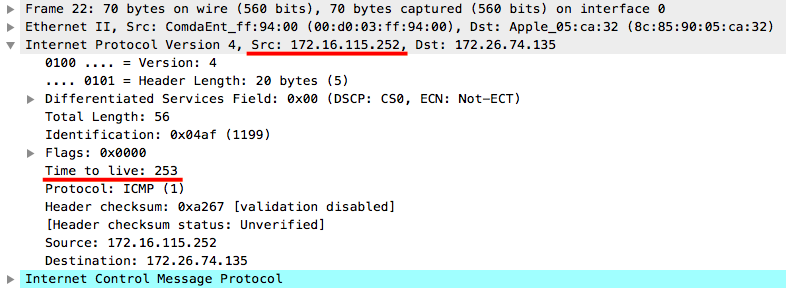
\includegraphics[scale=0.45]{2_g_3.png} 
\end{center}
\caption{\label{fig:2_g_3}Frame 22.}
\end{figure}

\textbf{R:} O primeiro valor do campo TTL é 255, e mantêm-se enquanto a fonte for a mesma. Quando a fonte variar este campo é decrementado uma unidade. Isto deve-se ao facto de que cada router tem que assegurar que a mensagem ICMP chega ao seu destino, daí ter um valor tão alto para o TTL. O facto de ser decrementado deve-se ao normal funcionamento de trânsito de datagramas entre routers, cada router diferente decrementa uma unidade ao TTL até este chegar ao destino. Como podemos ver nas imagens \ref{fig:2_g_1}, \ref{fig:2_g_2} e \ref{fig:2_g_3}, o TTL diminui consoante a Source.

\subsection{Exercício 3}
\emph{Pretende-se agora analisar a 
fragmentação de
pacotes
IP. 
Reponha a ordem
do 
tráfego  capturado
usando  a  coluna  do  tempo
de  captura. 
Observe  o  tráfego 
depois do tamanho de
pacote ter sido definido para 35XX bytes.  }

\subsubsection{a.}
\emph{Localize
a primeira mensagem 
ICMP. Porque 
é que 
houve
necessidade de 
fragmentar o pacote inicial
?}
\\ \par
\textbf{R:} A quantidade máxima de dados que um frame da camada Física consegue transportar chama-se  \textbf{MTU} (maximum transmission unit). Como os frames Ethernet só conseguem carregar até 1500 bytes de dados, e como nós queríamos capturar tráfego para pacotes com 3547 bytes, então ter-se-ia que se dividir o pacote inicial em 3 fragmentos.

\subsubsection{b.}
\emph{Imprima  o  primeiro  fragmento  do  datagrama  IP  segmentado.  Que 
informação no cabeçalho indica que o datagrama foi fragmentado? Que 
informação no cabeçalho IP indica 
que 
se trata do primeiro
fragmento
?
Qual é o tamanho 
deste data
grama IP
?}

\begin{figure}[H]
\begin{center}
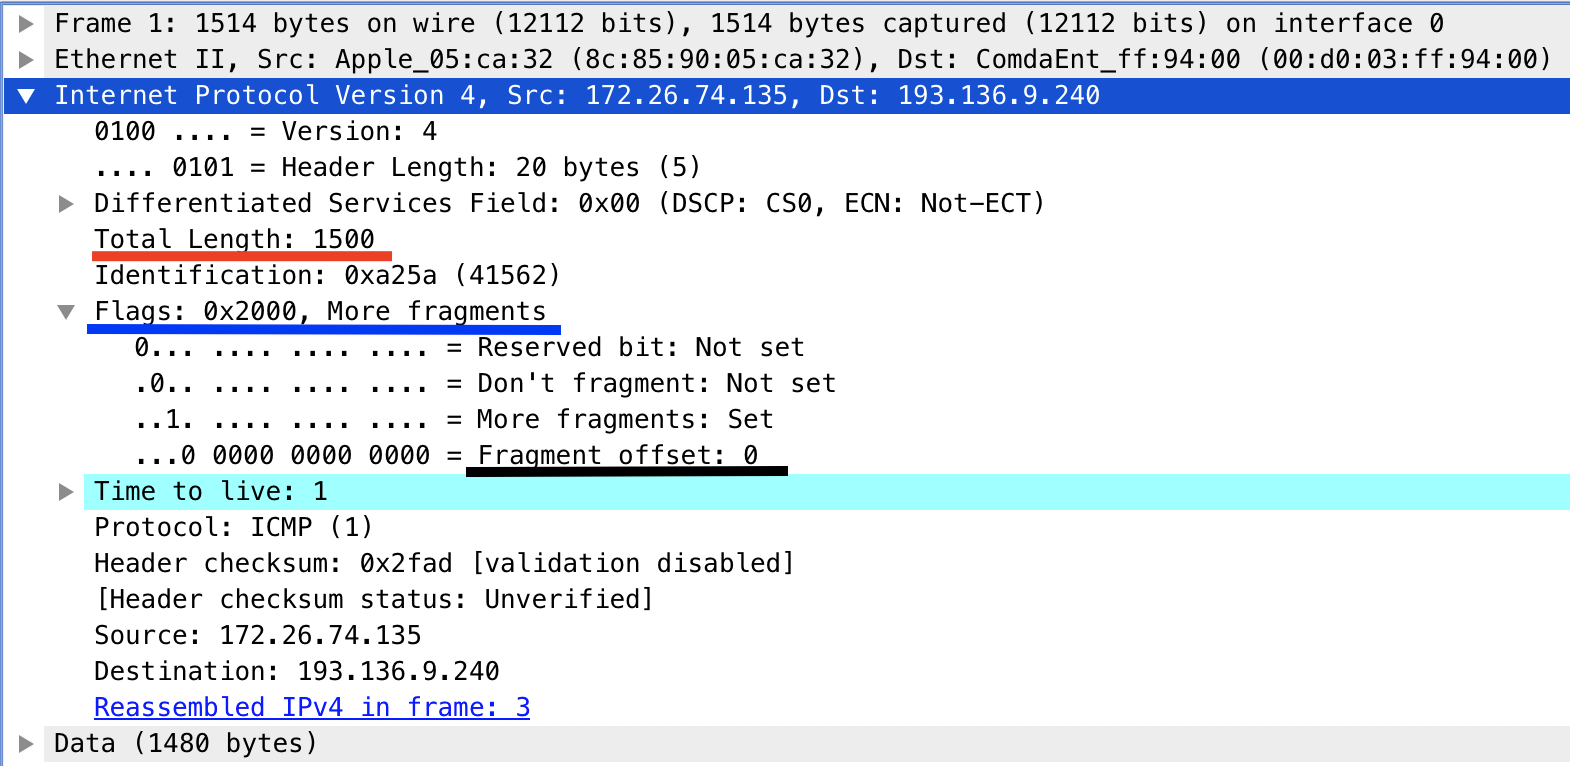
\includegraphics[scale=0.45]{3_b.png} 
\end{center}
\caption{\label{fig:3_b}Primeiro segmento do datagrama fragmentado.}
\end{figure}

\textbf{R:} Como se pode observar na figura \ref{fig:3_b}, sublinhado a azul escuro, existe uma flag no cabeçalho que indica a existência de mais fragmentos, se existem mais é porque o que está a ser analisado é um fragmento.

Trata-se do primeiro fragmento uma vez que o campo sublinhado a preto \textbf{Fragment offset}, indica o offset do datagrama e este está a 0. Segmentos consecutivos terão o campo do offset com valores maiores.

Como se pode observar na figura, sublinhado a vermelho, encontra-se o tamanho do datagrama que é \textbf{1500 bytes}.

\subsubsection{c.}
\emph{Imprima o 
segundo fragmento do datagrama 
IP
original
. Que informação 
do  cabeçalho  IP  indica  que  não  se  trata  do  1º  fragmento?  Há  mais 
fragmentos? O que nos permite afirmar isso?}

\begin{figure}[H]
\begin{center}
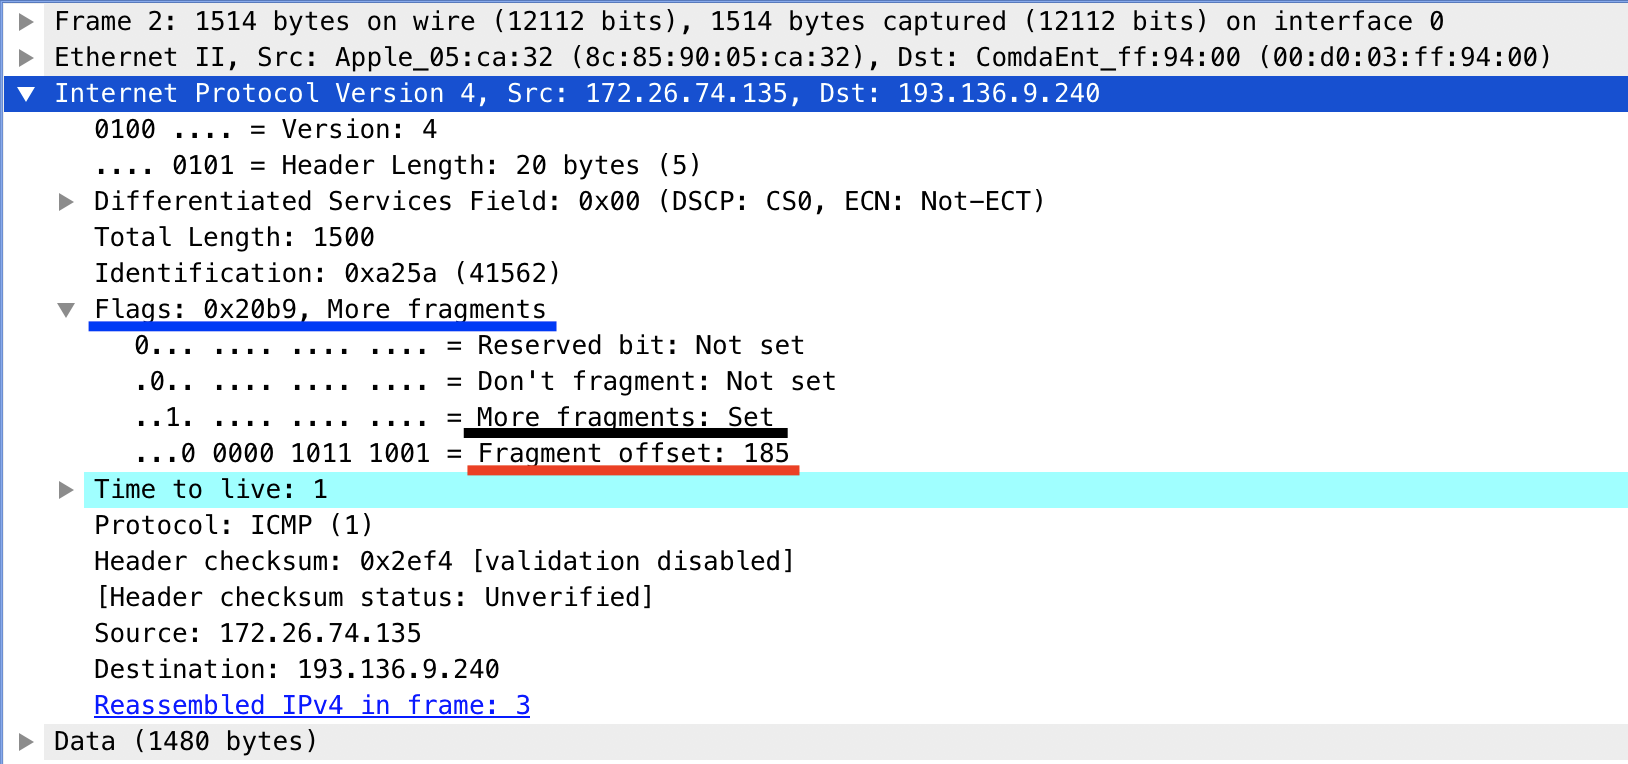
\includegraphics[scale=0.45]{3_c.png} 
\end{center}
\caption{\label{fig:3_c}Segundo segmento do datagrama fragmentado.}
\end{figure}

\textbf{R:} Existe no cabeçalho um campo que se denomina por Fragment offset, sublinhado a vermelho, que indica a posição do fragmento no datagrama original, basicamente é um campo que ajuda na tarefa de reagrupar os fragmentos aquando da chegada ao destino. Uma vez que o \textbf{Fragment offset} é 185, logicamente é diferente de 0 pelo que não se trata do primeiro fragmento.

Existem mais fragmentos, como se pode constatar na figura \ref{fig:3_c}, sublinhado a azul existe uma flag que indica a existência de mais fragmentos. Essa flag corresponde ao campo \textbf{More fragments}, sublinhado a preto, que está assinalado como verdadeiro.

\subsubsection{d.}
\emph{Quantos fragmentos foram criados a partir do datagrama original?
Como se detecta o último fragmento correspondente ao datagrama original?}

\begin{figure}[H]
\begin{center}
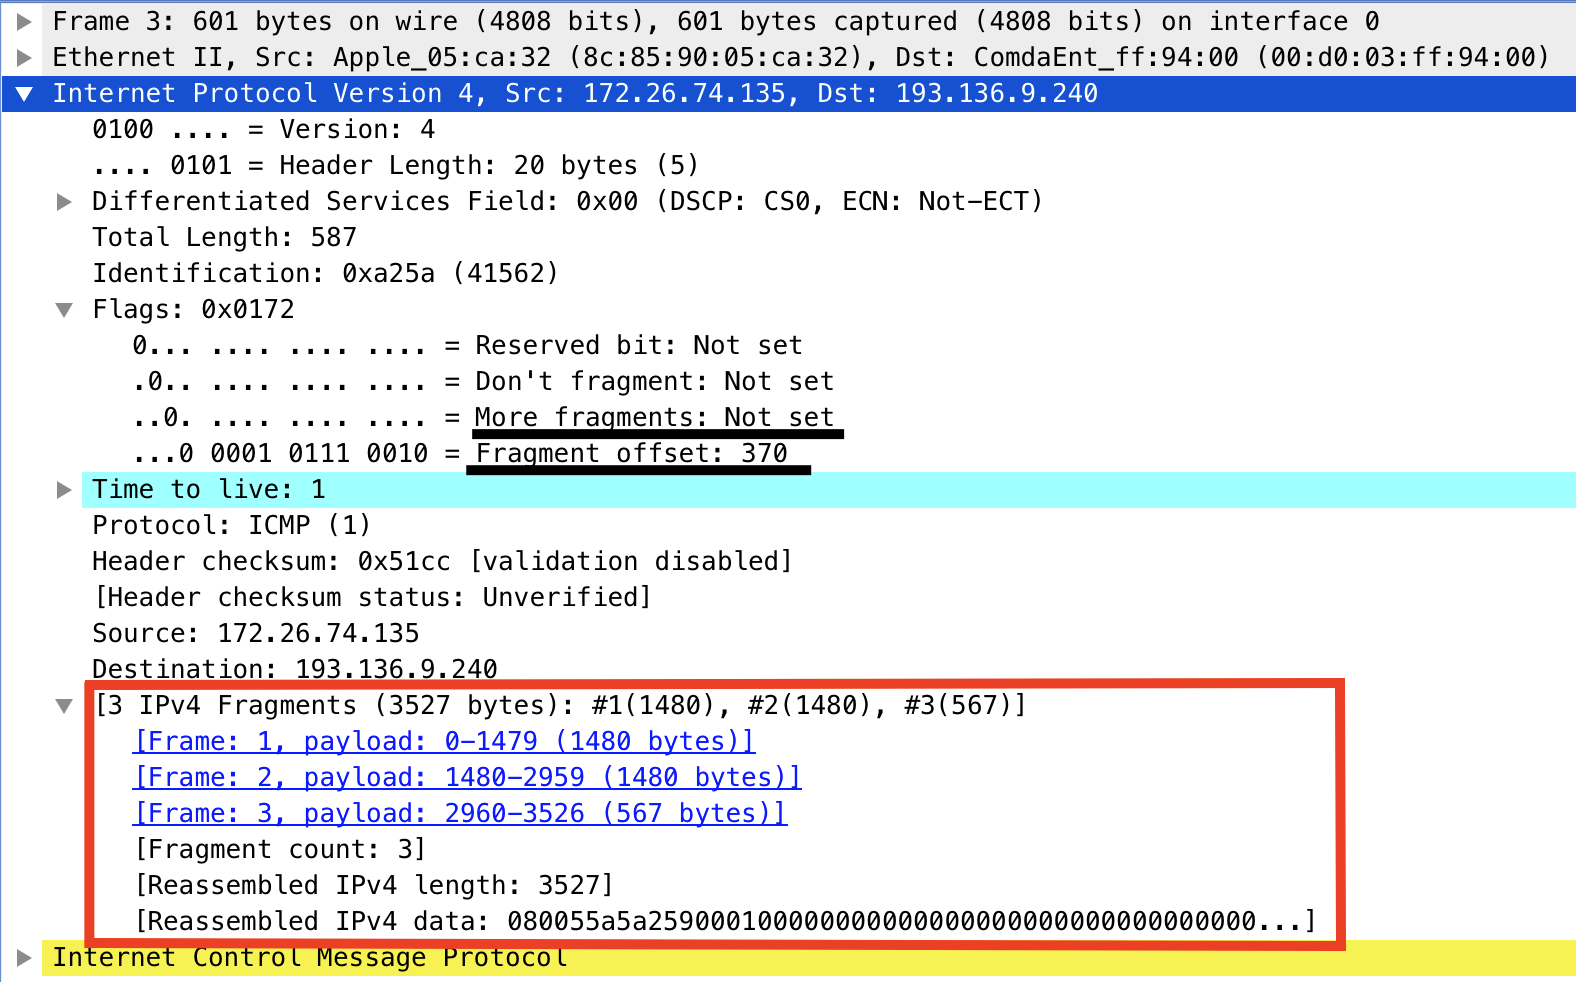
\includegraphics[scale=0.40]{3_d.png} 
\end{center}
\caption{\label{fig:3_d}Terceiro segmento do datagrama fragmentado.}
\end{figure}

\textbf{R:} Como se pode observar na figura \ref{fig:3_d}, no quadrado com contorno a vermelho, foram criados 3 fragmentos, aliás como se pode constatar no campo \textbf{Fragments count}, mas esta é informação que é fornecida pelo Wireshark e não está presente no cabeçalho IP.

O último fragmento do datagrama original pode ser identificado quando o campo \textbf{More fragments} não está assinalado(Not set), e quando o campo \textbf{Fragment offset} é diferente de 0. Observando a figura, assinalado a preto temos esses dois campos, que estão de acordo com o descrito. O campo \textbf{More fragments} não está assinalado e o campo \textbf{Fragment offset} é 370, que é logicamente diferente de 0.

\subsubsection{e.}
\emph{Indique, resumindo,
os
campos 
que 
mudam  no  cabeçalho  IP
entre  os 
diferentes fragmentos, e 
explique
a forma como essa informação permite 
reconstruir o datagrama original.}

\begin{figure}[H]
\begin{center}
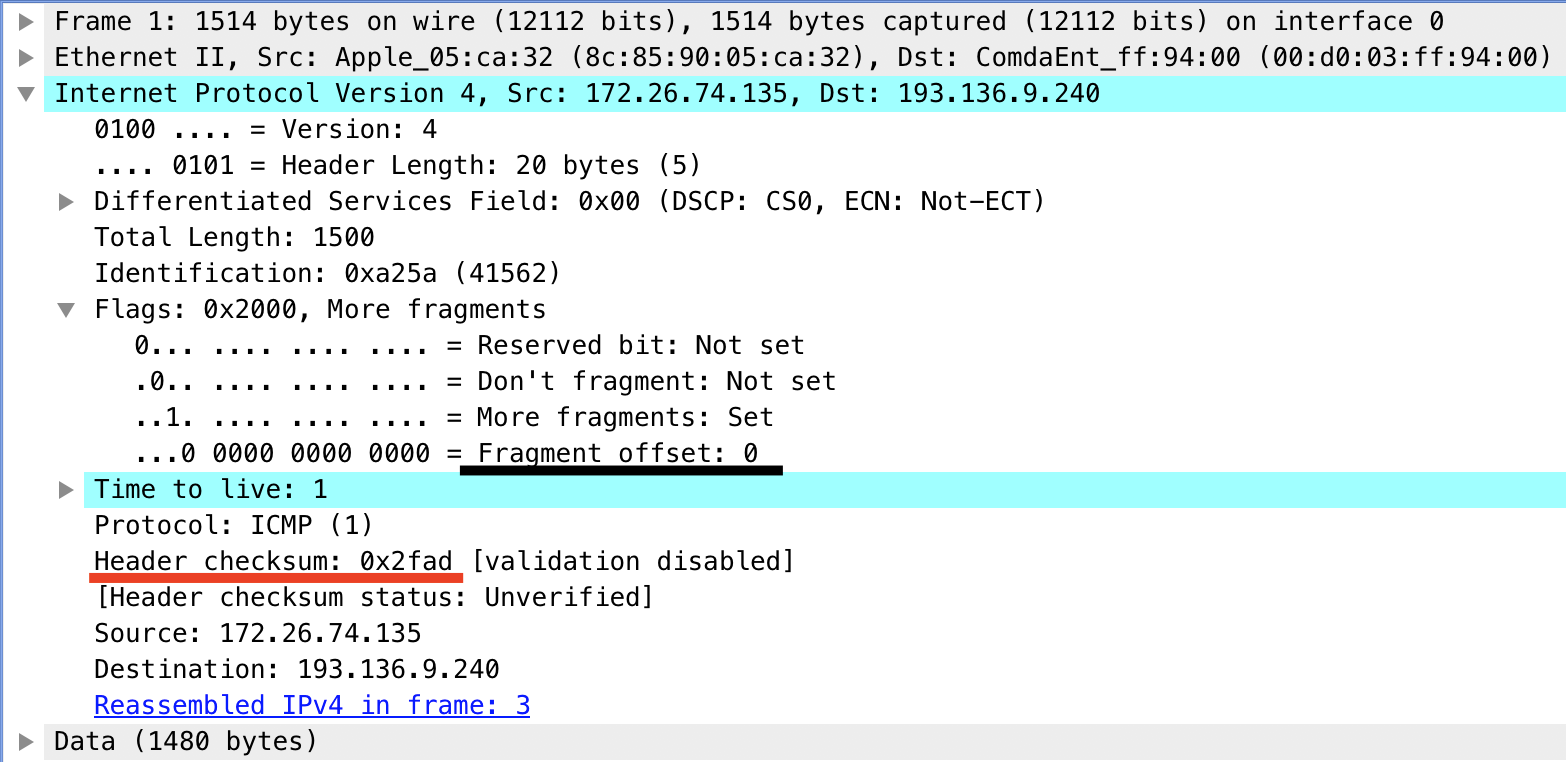
\includegraphics[scale=0.40]{3_e1.png} 
\end{center}
\caption{\label{fig:3_e1}Primeiro segmento do datagrama fragmentado.}
\end{figure}

\begin{figure}[H]
\begin{center}
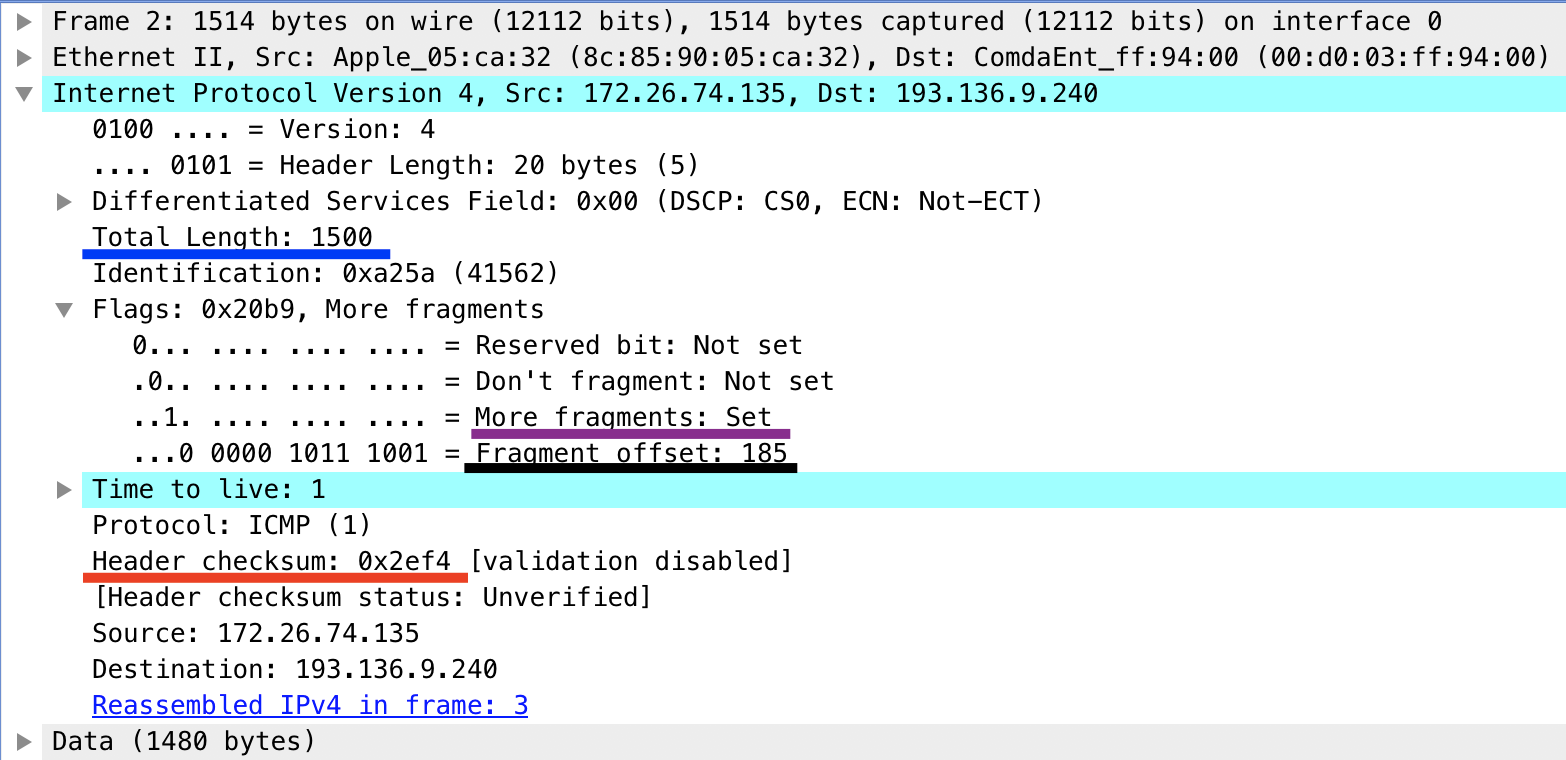
\includegraphics[scale=0.40]{3_e2.png} 
\end{center}
\caption{\label{fig:3_e2}Segundo segmento do datagrama fragmentado.}
\end{figure}

\begin{figure}[H]
\begin{center}
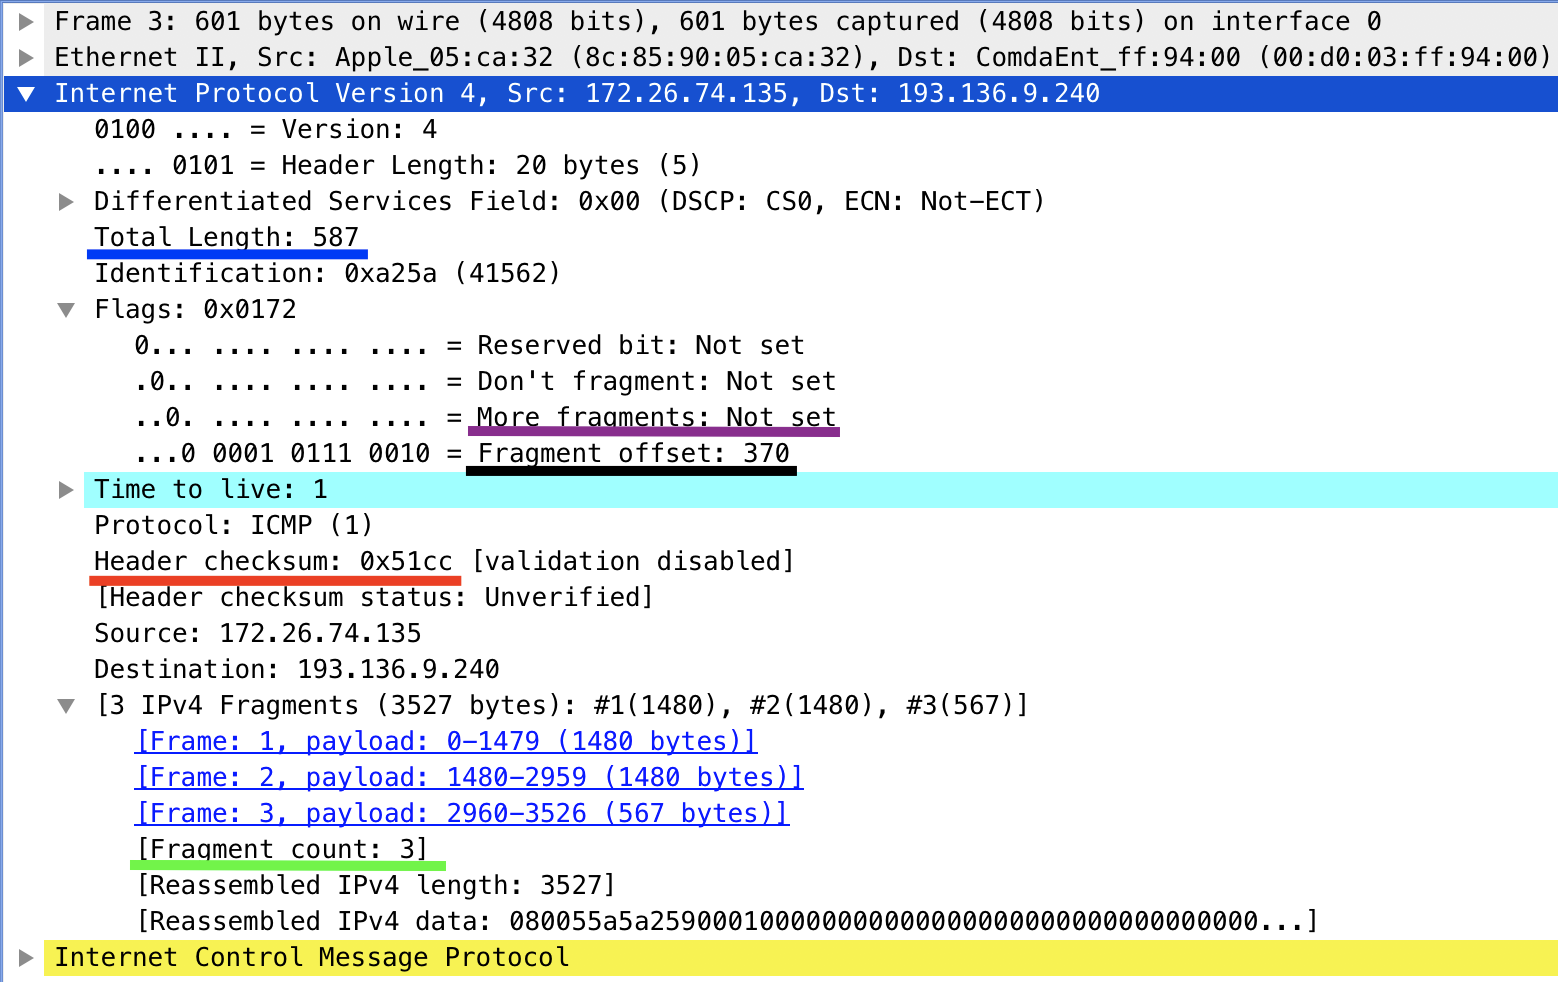
\includegraphics[scale=0.40]{3_e3.png} 
\end{center}
\caption{\label{fig:3_e3}Terceiro segmento do datagrama fragmentado.}
\end{figure}


\textbf{R:} Uma vez que existem 3 fragmentos relativos ao datagrama original podemos comparar os primeiros dois devido às suas semelhanças e por fim comparar as principais diferenças de um dos dois primeiros fragmentos para com o último fragmento.

Comparando os dois primeiros fragmentos, figura \ref{fig:3_e1} e \ref{fig:3_e2}, podemos notar que as principais diferenças estão nos campos \textbf{Fragment offset} e no \textbf{Header checksum}, que se encontram sublinhados em cada figura a preto e vermelho, respetivamente.

Comparando o segundo fragmento com o último, figura \ref{fig:3_e2} e \ref{fig:3_e3}, as principais diferenças estão nos campos \textbf{Total Length}, \textbf{More fragments}, \textbf{Fragment offset} e no \textbf{Header checksum}, que se encontram sublinhados em cada figura a azul, roxo, preto e vermelho, respetivamente.

O campo \textbf{Identification} é igual em todos os fragmentos pelo que no destino é possível saber quais dos fragmentos vão originar um datagrama. O campo  \textbf{More fragments} dita se ainda existem mais fragmentos, sabe-se então que se recebe o último fragmento quando este campo não está assinalado (Not set). Este último fragmento permite observar, como se pode constatar na figura \ref{fig:3_e3}, no campo  \textbf{Fragment count} sublinhado a verde, em quantos fragmentos foi dividido o datagrama original, pelo que se consegue saber se já foram recebidos todos os fragmentos ou não. Por último, depois de todos os fragmentos chegarem ao destino, para reconstruir o datagrama original por ordem usa-se o campo  \textbf{Fragment offset}, que dita em que posição cada fragmento se encontra no datagrama original.


\end{document}